\documentclass[12pt, a4paper]{article}

\usepackage[margin=1in]{geometry}
\usepackage{amsmath, amssymb, amsthm}
\usepackage{graphicx}
\usepackage{hyperref}
\usepackage{enumitem}
\usepackage{float}
\usepackage{xcolor}
\usepackage{listings}

\lstset{
    basicstyle=\ttfamily\scriptsize,
    backgroundcolor=\color{gray!10},
    frame=single,
    breaklines=true,
    columns=flexible,
    keepspaces=true
}

\title{18-786: Introduction to Deep Learning \\ Homework 4: Convolutional Neural Networks}
\author{Qinglang Wang (Andrew ID: qinglang)}
\date{\today}

\begin{document}

\maketitle

\section{Object Classification with CIFAR-100 Dataset}

\subsection*{Fully Connected Neural Network (FCNN)}

\subsubsection*{(a) Model Architecture}
The FCNN model takes flattened $3 \times 32 \times 32$ images and processes them through three hidden layers.
\begin{lstlisting}
FCNN(
  (layers): Sequential(
    (0): Linear(in_features=3072, out_features=1024, bias=True)
    (1): BatchNorm1d(1024, eps=1e-05, momentum=0.1, affine=True, track_running_stats=True)
    (2): ReLU()
    (3): Dropout(p=0.4, inplace=False)
    (4): Linear(in_features=1024, out_features=512, bias=True)
    (5): BatchNorm1d(512, eps=1e-05, momentum=0.1, affine=True, track_running_stats=True)
    (6): ReLU()
    (7): Dropout(p=0.4, inplace=False)
    (8): Linear(in_features=512, out_features=256, bias=True)
    (9): BatchNorm1d(256, eps=1e-05, momentum=0.1, affine=True, track_running_stats=True)
    (10): ReLU()
    (11): Dropout(p=0.4, inplace=False)
    (12): Linear(in_features=256, out_features=100, bias=True)
  )
)
\end{lstlisting}


\subsubsection*{(b) Hyper-parameters}
\begin{lstlisting}
Config(
    Optimizer: Adam,
    Learning Rate: 4e-3,
    Weight Decay: 1e-3,
    Learning Rate Scheduler: Cosine Annealing,
    Batch Size: 512,
    Epochs: 50,
    Dropout Rate: 0.4
)
\end{lstlisting}

\subsubsection*{(c) Performance}
The FCNN achieved a maximum validation accuracy of \textbf{31.88\%}.

\begin{figure}[H]
    \centering
    \begin{minipage}{0.48\textwidth}
        \centering
        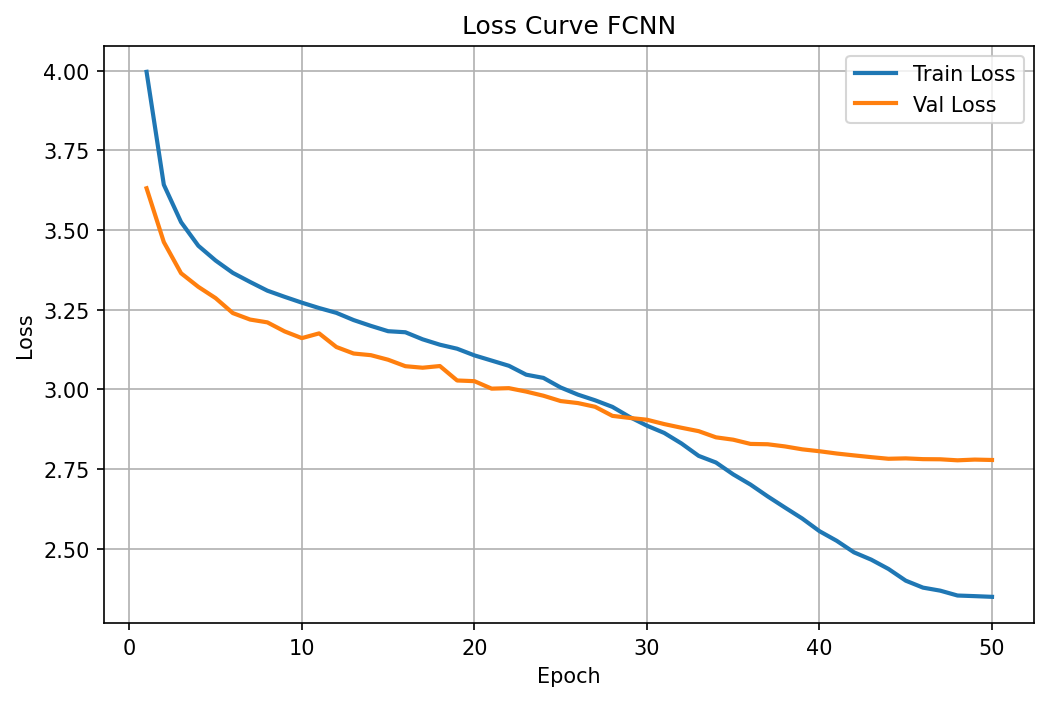
\includegraphics[width=\linewidth]{results/q1_fcnn_loss.png}
        \caption{FCNN Train/Test Losses}
    \end{minipage}\hfill
    \begin{minipage}{0.48\textwidth}
        \centering
        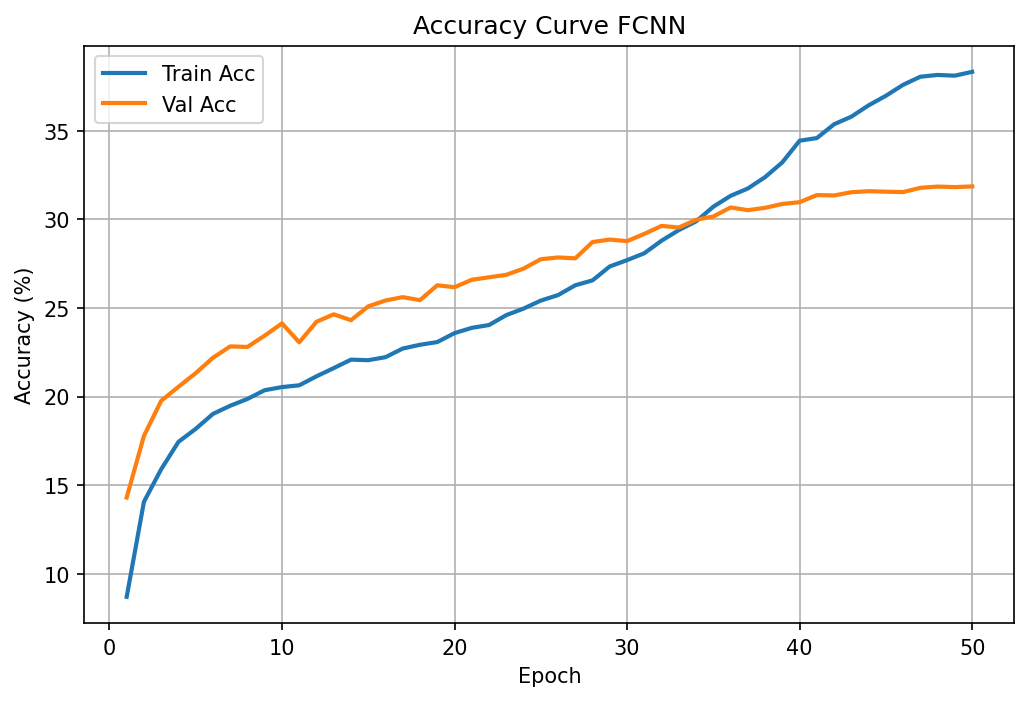
\includegraphics[width=\linewidth]{results/q1_fcnn_acc.png}
        \caption{FCNN Train/Test Accuracies}
    \end{minipage}
\end{figure}

\begin{figure}[H]
    \centering
    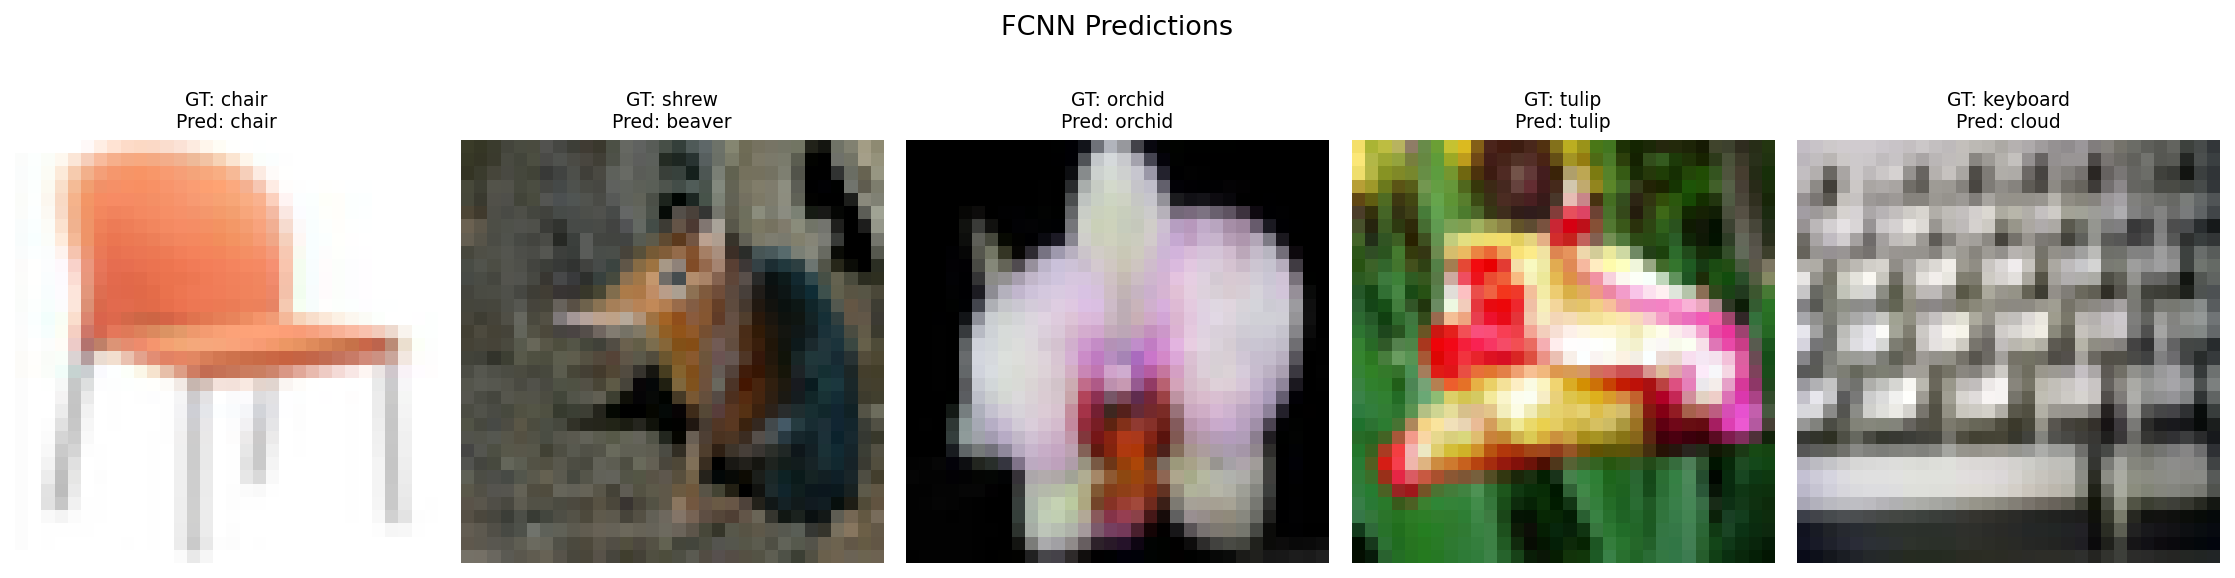
\includegraphics[width=\linewidth]{results/q1_fcnn_preds.png}
    \caption{Visualization of FCNN predictions on 5 random images}
\end{figure}

\begin{figure}[H]
    \centering
    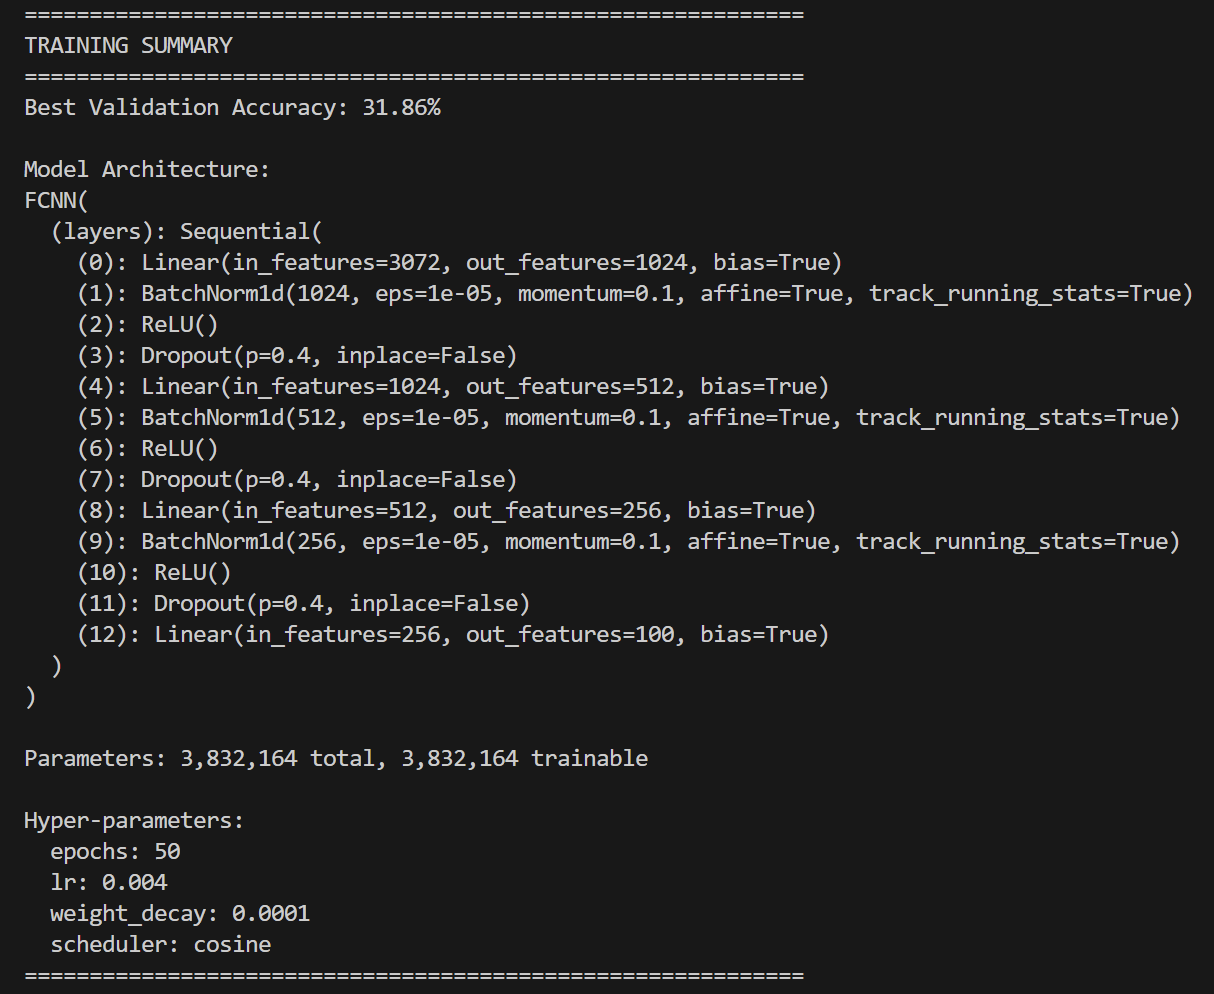
\includegraphics[width=\linewidth]{results/q1_fcnn_summary.png}
    \caption{FCNN Training Log}
\end{figure}

\subsection*{Convolutional Neural Network (CNN)}
\subsubsection*{(a) Model Architecture}
The CNN model utilizes custom \texttt{MyConv2D} and \texttt{MyMaxPool2D} layers.
\begin{lstlisting}
CNN(
  (backbone): Sequential(
    (0): MyConv2D(3, 32, kernel_size=(3, 3), stride=(1, 1), padding=(1, 1))
    (1): BatchNorm2d(32)
    (2): ReLU()
    (3): MyConv2D(32, 64, kernel_size=(3, 3), stride=(1, 1), padding=(1, 1))
    (4): BatchNorm2d(64)
    (5): ReLU()
    (6): MyMaxPool2D(kernel_size=2, stride=2)
    (7): MyConv2D(64, 128, kernel_size=(3, 3), stride=(1, 1), padding=(1, 1))
    (8): BatchNorm2d(128)
    (9): ReLU()
    (10): MyMaxPool2D(kernel_size=2, stride=2)
    (11): MyConv2D(128, 256, kernel_size=(3, 3), stride=(1, 1), padding=(1, 1))
    (12): BatchNorm2d(256)
    (13): ReLU()
    (14): AdaptiveAvgPool2d(output_size=1)
  )
  (head): Linear(in_features=256, out_features=100, bias=True)
)
\end{lstlisting}

\subsubsection*{(b) Hyper-parameters}
\begin{lstlisting}
Config(
    Optimizer: Adam,
    Learning Rate: 3e-3,
    Weight Decay: 1e-4,
    Learning Rate Scheduler: Cosine Annealing,
    Batch Size: 512,
    Epochs: 10
)
\end{lstlisting}

\subsubsection*{(c) Performance}
The CNN achieved a maximum validation accuracy of \textbf{50.80\%}.

\begin{figure}[H]
    \centering
    \begin{minipage}{0.48\textwidth}
        \centering
        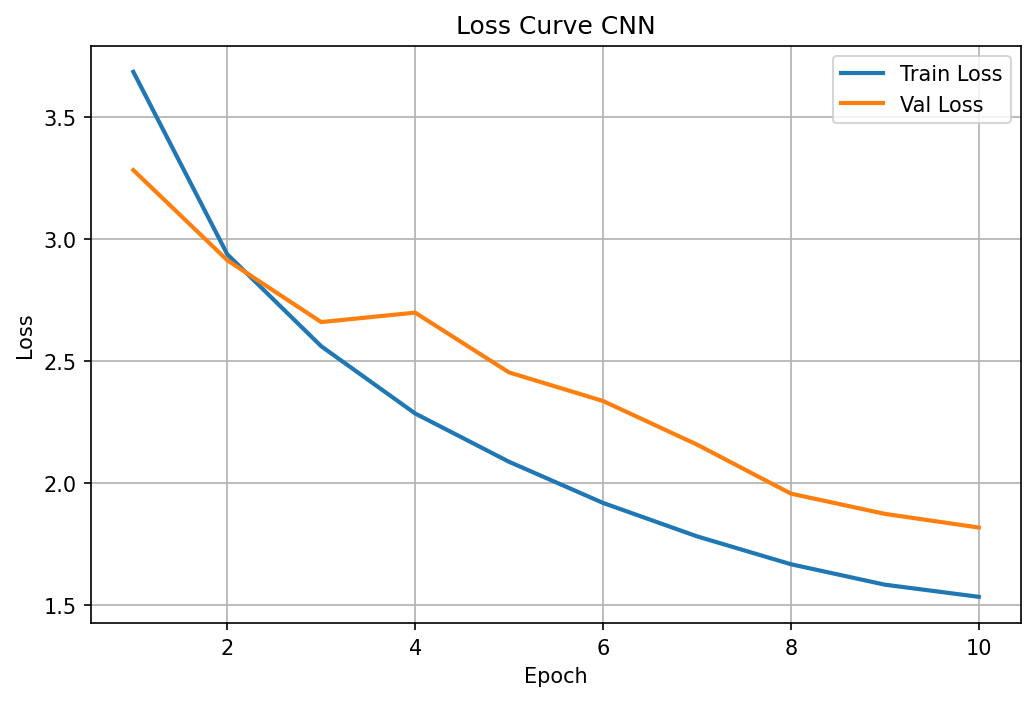
\includegraphics[width=\linewidth]{results/q1_cnn_loss.png}
        \caption{CNN Train/Test Losses}
    \end{minipage}\hfill
    \begin{minipage}{0.48\textwidth}
        \centering
        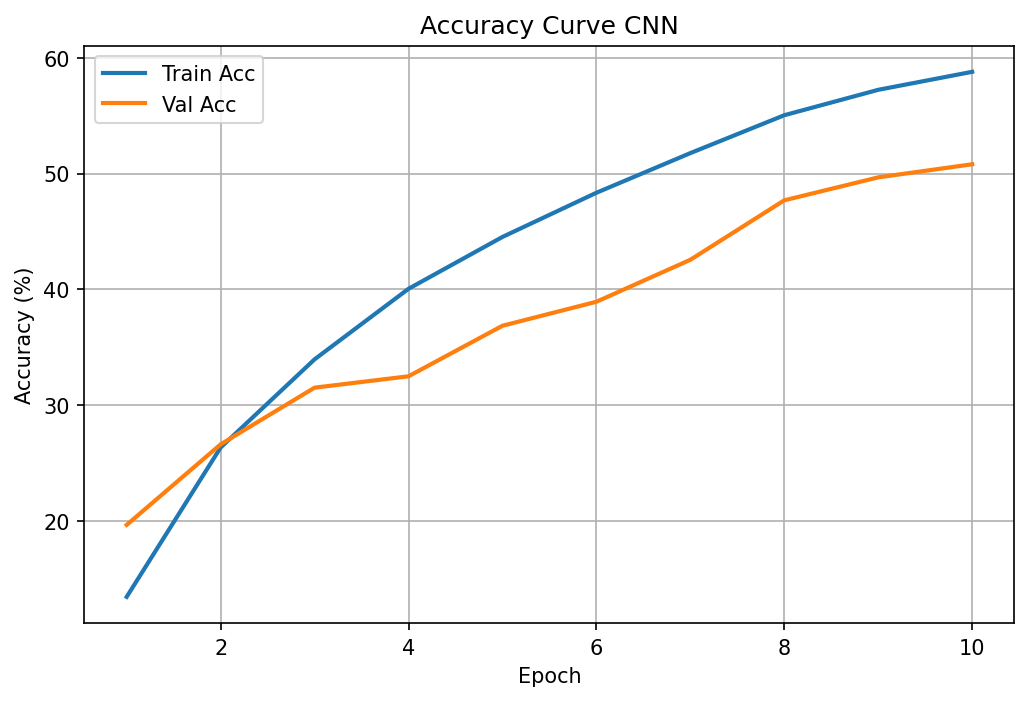
\includegraphics[width=\linewidth]{results/q1_cnn_acc.png}
        \caption{CNN Train/Test Accuracies}
    \end{minipage}
\end{figure}

\begin{figure}[H]
    \centering
    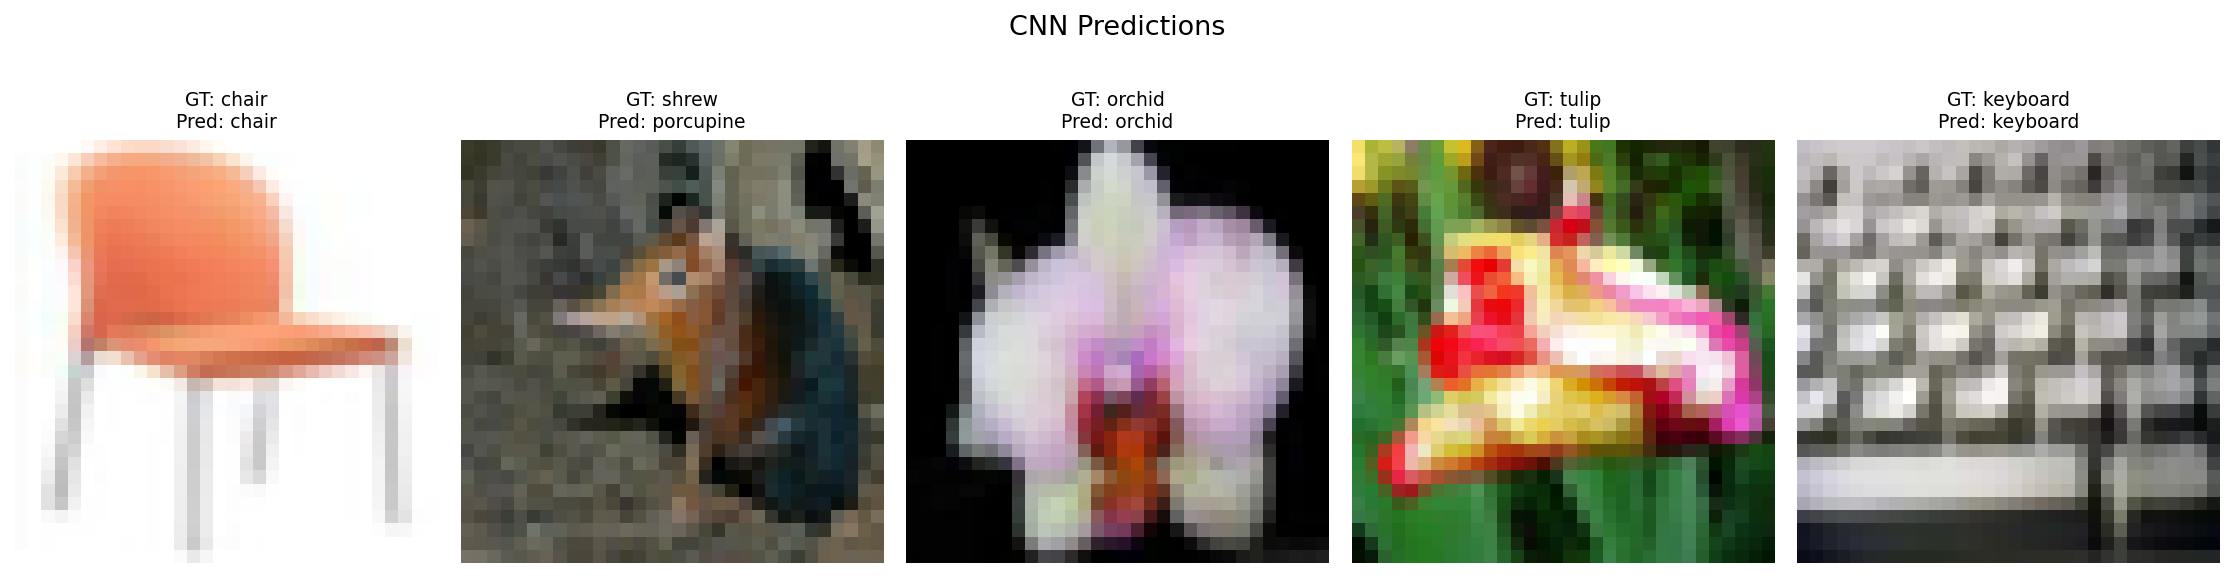
\includegraphics[width=\linewidth]{results/q1_cnn_preds.png}
    \caption{Visualization of CNN predictions on 5 random images}
\end{figure}

\begin{figure}[H]
    \centering
    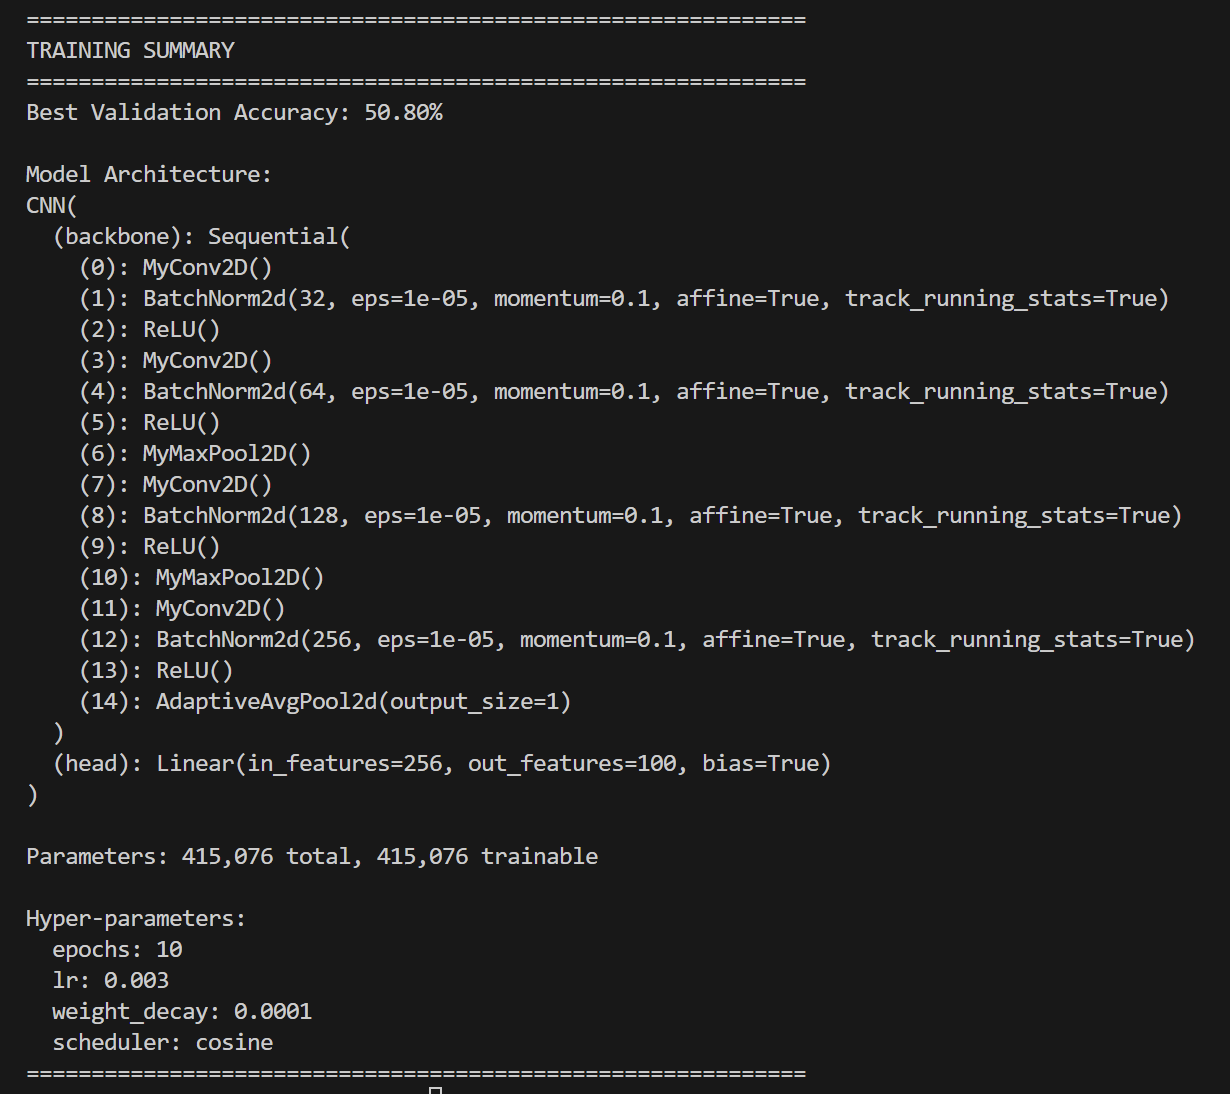
\includegraphics[width=\linewidth]{results/q1_cnn_summary.png}
    \caption{CNN Training Log}
\end{figure}

\subsection*{Learnings and Insights}

There are 2 main concerns I would like to emphasize:
\begin{itemize}
    \item \textbf{Training Stability}: To stabilize the training process and reach higher accuracies, learning rate scheduling (Cosine Annealing) greatly improved optimization compared to a fixed learning rate. Moreover, I try to introduce Batch Normalization to stabilize the inputs, which also contributes to performance improvement.
    \item \textbf{Overfitting}: Dropout rates in the FCNN were tuned to $0.4$. The lower dropout rate will lead to rapid overfitting of the training data, while the higher value will lead to slow convergence.
\end{itemize}
In conclusion, the spatial structural perception capability harnessed by convolutions proved very powerful, obtaining much stronger performance despite executing for only 10 epochs.

\section{Training for Optimal Results}

\subsection*{Deep Residual Network (ResNet18)}

\subsubsection*{(a) Model Architecture}
The ResNet18 is built upon the \texttt{ResidualBlock}.

\begin{lstlisting}
ResidualBlock(in_channels, out_channels, stride)
  (conv1): Conv2d(in_channels, out_channels, kernel_size=(3, 3), stride=(stride, stride), padding=(1, 1), bias=False)
  (bn1): BatchNorm2d(out_channels, eps=1e-05, momentum=0.1, affine=True, track_running_stats=True)
  (conv2): Conv2d(out_channels, out_channels, kernel_size=(3, 3), stride=(1, 1), padding=(1, 1), bias=False)
  (bn2): BatchNorm2d(out_channels, eps=1e-05, momentum=0.1, affine=True, track_running_stats=True)
  if stride != 1 or in_channels != out_channels:
    (downsample): Sequential(
      (0): Conv2d(in_channels, out_channels, kernel_size=(1, 1), stride=(stride, stride), bias=False)
      (1): BatchNorm2d(out_channels, eps=1e-05, momentum=0.1, affine=True, track_running_stats=True)
  )
ResNet18(
  (conv1): Conv2d(3, 64, kernel_size=(3, 3), stride=(1, 1), padding=(1, 1), bias=False)
  (bn1): BatchNorm2d(64, eps=1e-05, momentum=0.1, affine=True, track_running_stats=True)
  (layer1): Sequential(
    (0): ResidualBlock(in_channels=64, out_channels=64, stride=1)
    (1): ResidualBlock(in_channels=64, out_channels=64, stride=1)
  )
  (layer2): Sequential(
    (0): ResidualBlock(in_channels=64, out_channels=128, stride=2, downsample=True)
    (1): ResidualBlock(in_channels=128, out_channels=128, stride=1)
  )
  (layer3): Sequential(
    (0): ResidualBlock(in_channels=128, out_channels=256, stride=2, downsample=True)
    (1): ResidualBlock(in_channels=256, out_channels=256, stride=1)
  )
  (layer4): Sequential(
    (0): ResidualBlock(in_channels=256, out_channels=512, stride=2, downsample=True)
    (1): ResidualBlock(in_channels=512, out_channels=512, stride=1)
  )
  (avgpool): AdaptiveAvgPool2d(output_size=1)
  (fc): Linear(in_features=512, out_features=100, bias=True)
)
\end{lstlisting}

\subsubsection*{(b) Hyper-parameters}
\begin{lstlisting}
Config(
    Optimizer: SGD with momentum = 0.9,
    Learning Rate: 3e-1,
    Weight Decay: 5e-4,
    Learning Rate Scheduler: Cosine Annealing,
    Data Augmentation: Enabled (Random Crop & Random Horizontal Flip),
    Batch Size: 512,
    Epochs: 100
)
\end{lstlisting}

\subsubsection*{(c) Performance}
The ResNet18 achieved a max validation accuracy of \textbf{76.89\%}.

\begin{figure}[H]
    \centering
    \begin{minipage}{0.48\textwidth}
        \centering
        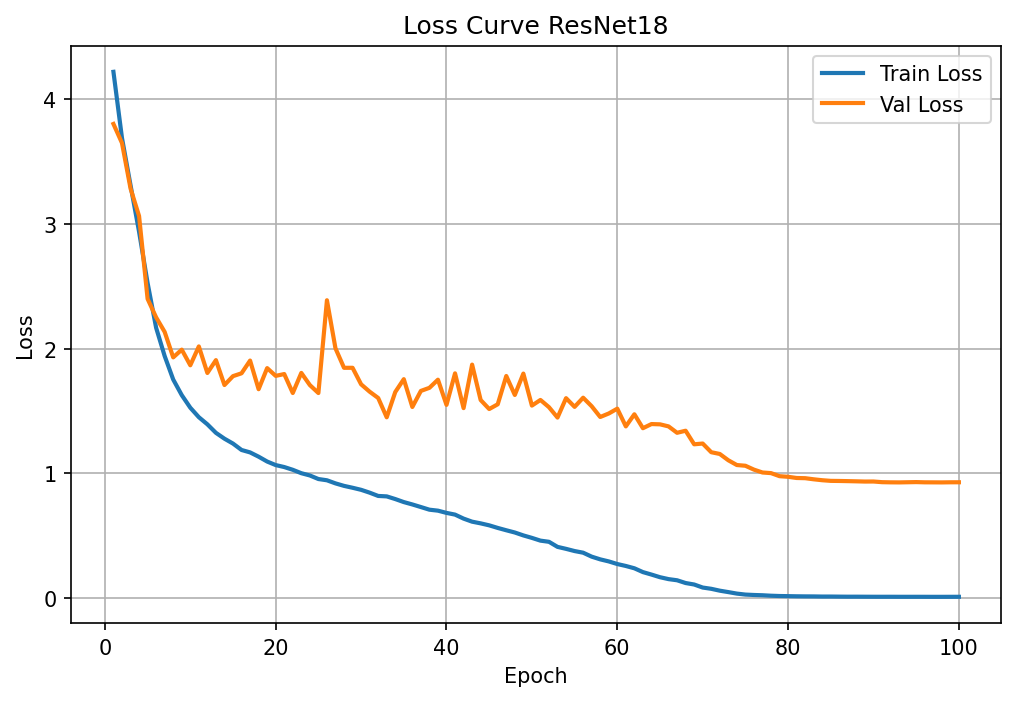
\includegraphics[width=\linewidth]{results/q2_resnet18_loss.png}
        \caption{ResNet Train/Test Losses}
    \end{minipage}\hfill
    \begin{minipage}{0.48\textwidth}
        \centering
        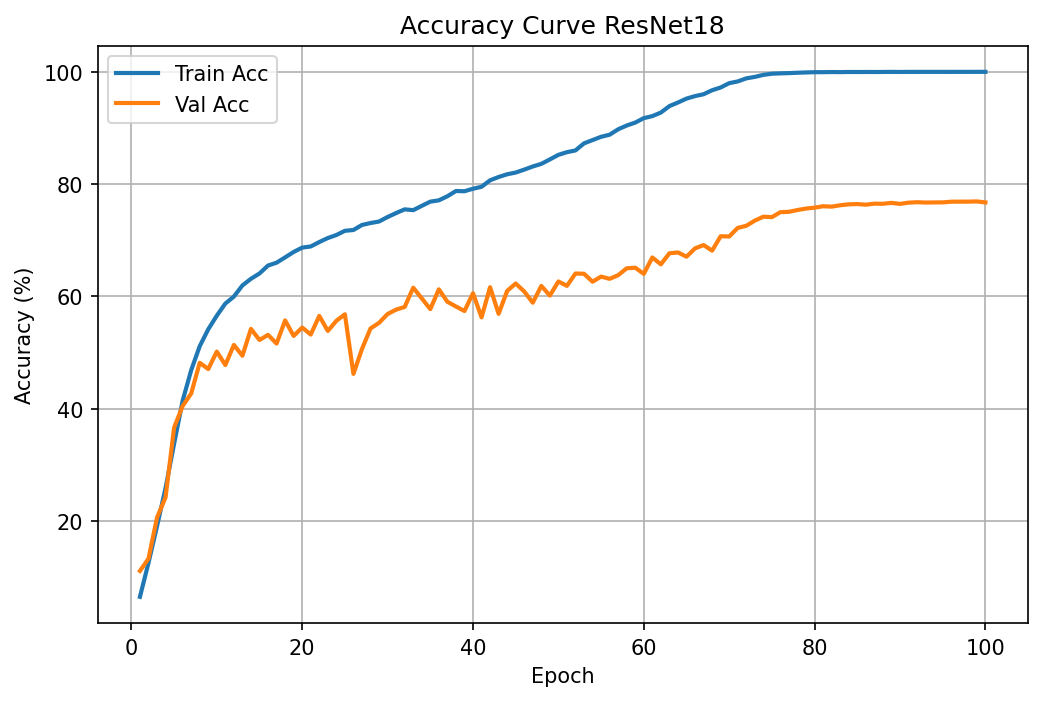
\includegraphics[width=\linewidth]{results/q2_resnet18_acc.png}
        \caption{ResNet Train/Test Accuracies}
    \end{minipage}
\end{figure}

\begin{figure}[H]
    \centering
    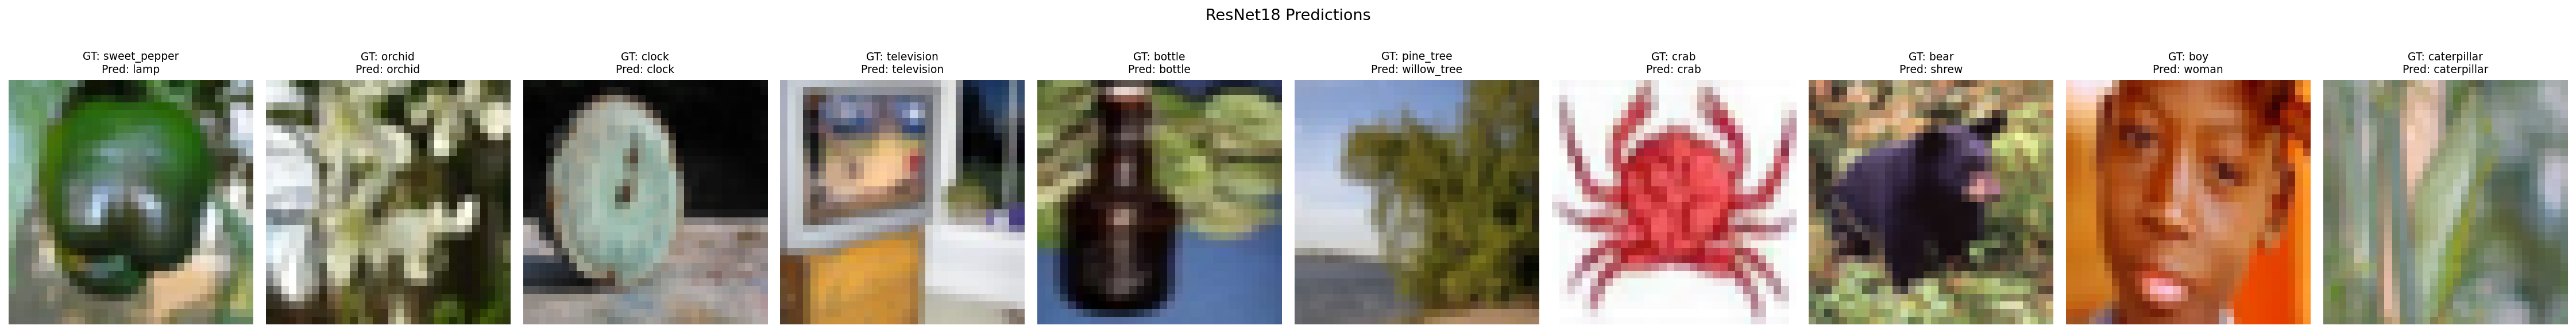
\includegraphics[width=\linewidth]{results/q2_resnet18_preds.png}
    \caption{Visualization of ResNet18 predictions out of 10}
\end{figure}

\subsubsection*{(D) Ablation Study, Learnings and Insights}
The following table summarizes the quantitative results of the ablation study conducted over 20 epochs to evaluate the impact of various enhancements on the ResNet18 model:

\begin{center}
\begin{tabular}{|l|c|c|}
    \hline
    \textbf{Configuration} & \textbf{Val Acc (20 eps)} & \textbf{Improvement} \\
    \hline
    Baseline (No Aug, Adam, LR=1e-3, WD=0) & 57.28\% & - \\
    + Data Augmentation & 68.29\% & \textbf{+11.01\%} \\
    + Switch to SGD (LR=0.1, M=0.9) & 66.95\% & -1.34\% \\
    + Add Weight Decay (5e-4) & 69.67\% & +2.72\% \\
    + LR Tuning (LR=0.3) & 70.91\% & +1.24\% \\
    \hline
\end{tabular}
\end{center}

\noindent Given the ablation results above, we can conclude the following learnings and insights:
\begin{itemize}
    \item \textbf{Data Augmentation} is the single most critical factor, providing a massive 11.01\% gain by effectively regularizing the model against overfitting.
    \item \textbf{Adam} converges faster initially, while \textbf{SGD with Weight Decay} provides more stable generalization in the long run. I adopted \textbf{SGD} for stability preference. And experiment shows that Adam achieves 74.07\% on the 100 epochs, lower than 76.89\% of SGD implementation.
    \item Tuning the \textbf{Learning Rate} to 0.3 (compatible with the Cosine Annealing scheduler) can contribute to extracting the final percentages of performance.
\end{itemize}
Avoiding rapid overfitting through these techniques allowed the model to reach a final accuracy of 76.89\% over 100 epochs.

\section{Naive Object Detection}

\subsection*{(a) Rigid Grid Baseline}
 For the basic implementation, images were equally divided into a standard $5\times5$ grid forming sub-image patches, classifying each isolated patch to see whether it contained a cat or dog if confidence exceeds the threshold.

\begin{figure}[H]
    \centering
    \begin{minipage}{0.48\textwidth}
        \centering
        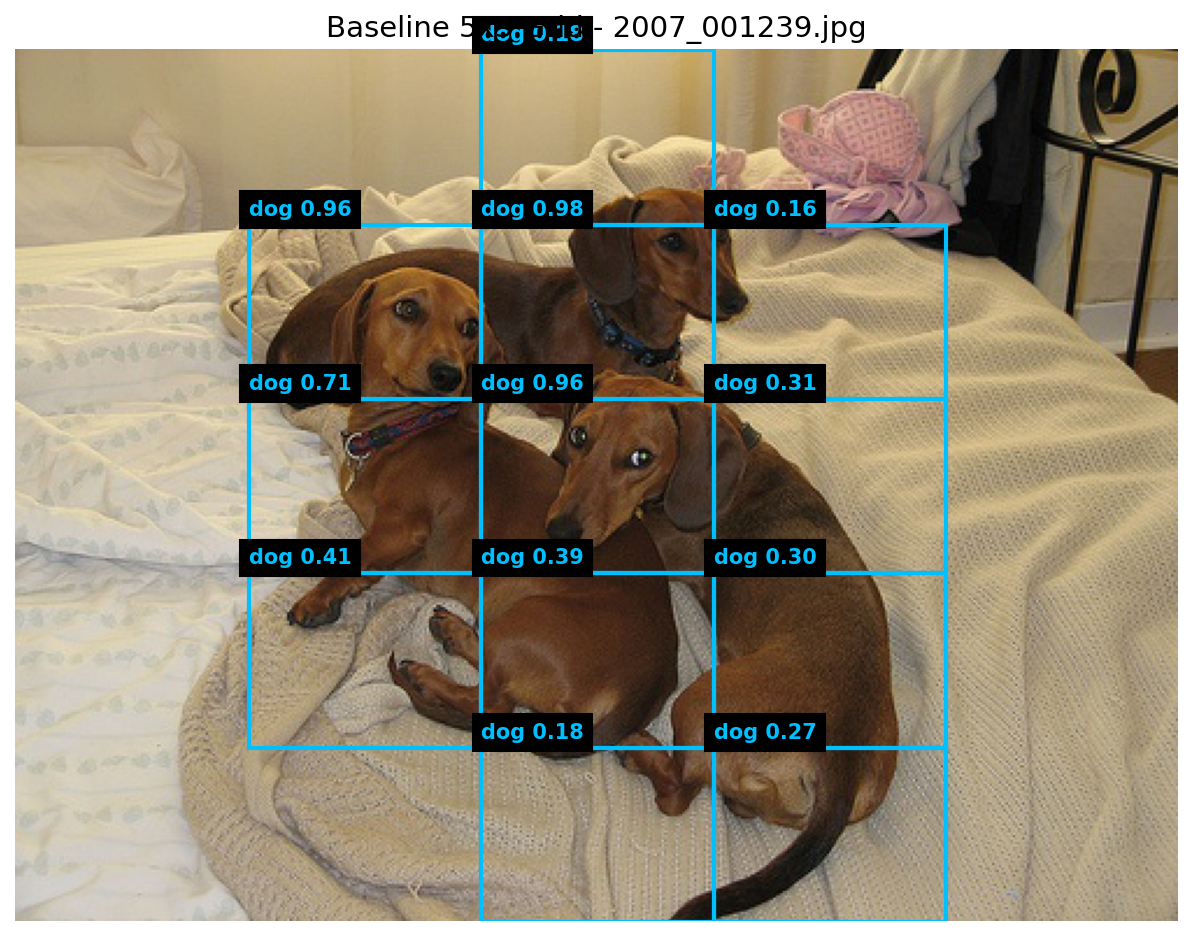
\includegraphics[width=\linewidth]{results/q3_baseline_2007_001239.png}
        \caption{Baseline on Image 1}
        \label{fig:12}
    \end{minipage}\hfill
    \begin{minipage}{0.48\textwidth}
        \centering
        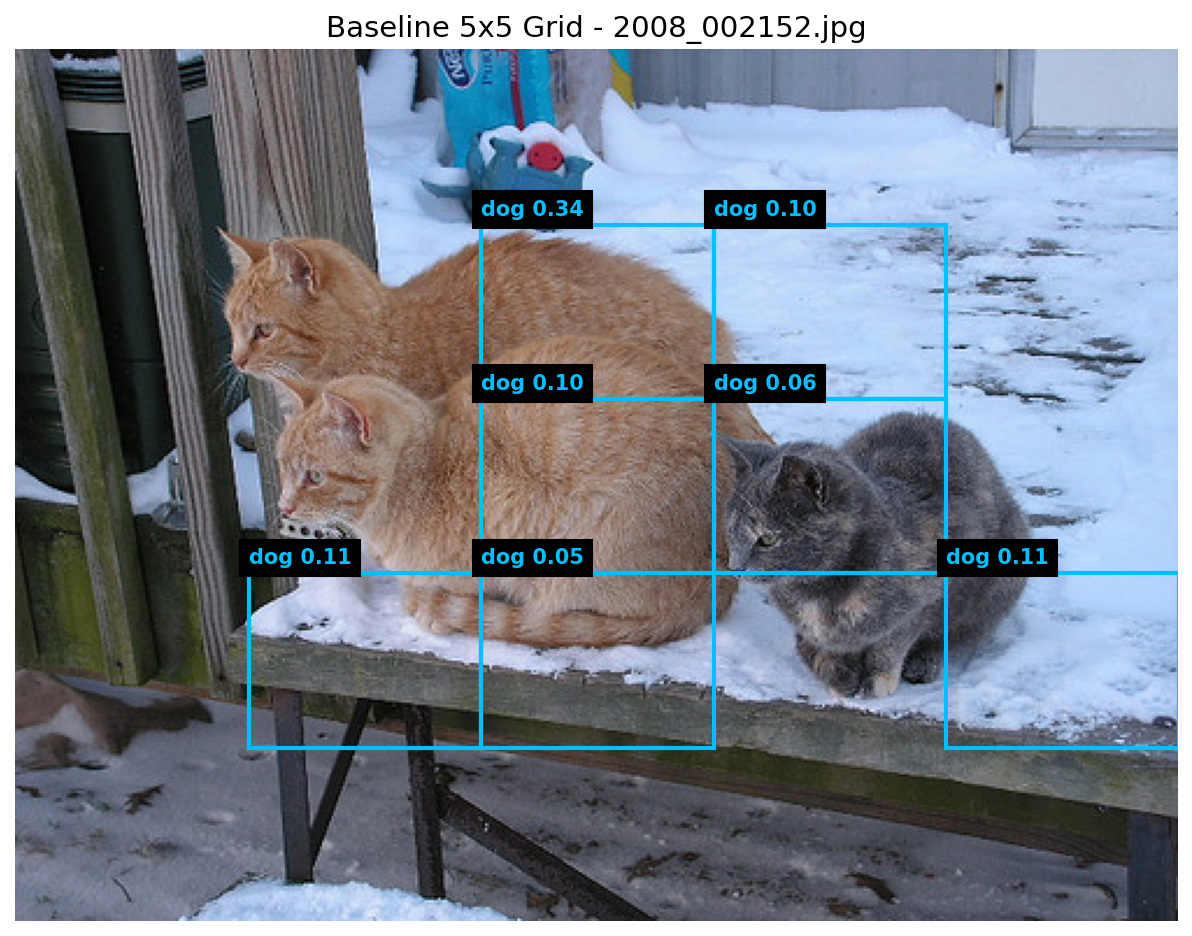
\includegraphics[width=\linewidth]{results/q3_baseline_2008_002152.png}
        \caption{Baseline on Image 2}
        \label{fig:13}
    \end{minipage}
\end{figure}

As we can see from Figs.\ref{fig:12} and \ref{fig:13}, the detection results of dogs are reasonable, but that of cats are really awful. This is due to the unbalanced classes of cats and dogs and also the fixed detection region scale.

\subsection*{(b) Multi-Scale Sliding Window Method}
To improve the limitation mentioned above, I implemented this \textbf{Multi-Scale Sliding Window Mechanism}:
\begin{itemize}
    \item \textbf{Crop Variations:} Instead of static non-overlapping patches, patches of assorted base sizes $[64, 96, 128, 160, 192, 224]$ combined with multiple aspect ratios $[0.5, 0.75, 1.0, 1.5, 2.0]$ generate continuously sliding windows across the entire image, which enables the detector to capture objects of different scales and postures.
    \item \textbf{Merging Sub-Images:} The method above generates tons of overlapping boxes over a single target. So I implemented the \textbf{Non-Maximum Suppression (NMS)} method and set the IoU threshold to $0.01$. By comparing every box pairs and keeping the one with higher classifier confidence, It effectively prunes thousands of redundant boxes overlapping similar components.
\end{itemize}

\begin{figure}[H]
    \centering
    \begin{minipage}{0.48\textwidth}
        \centering
        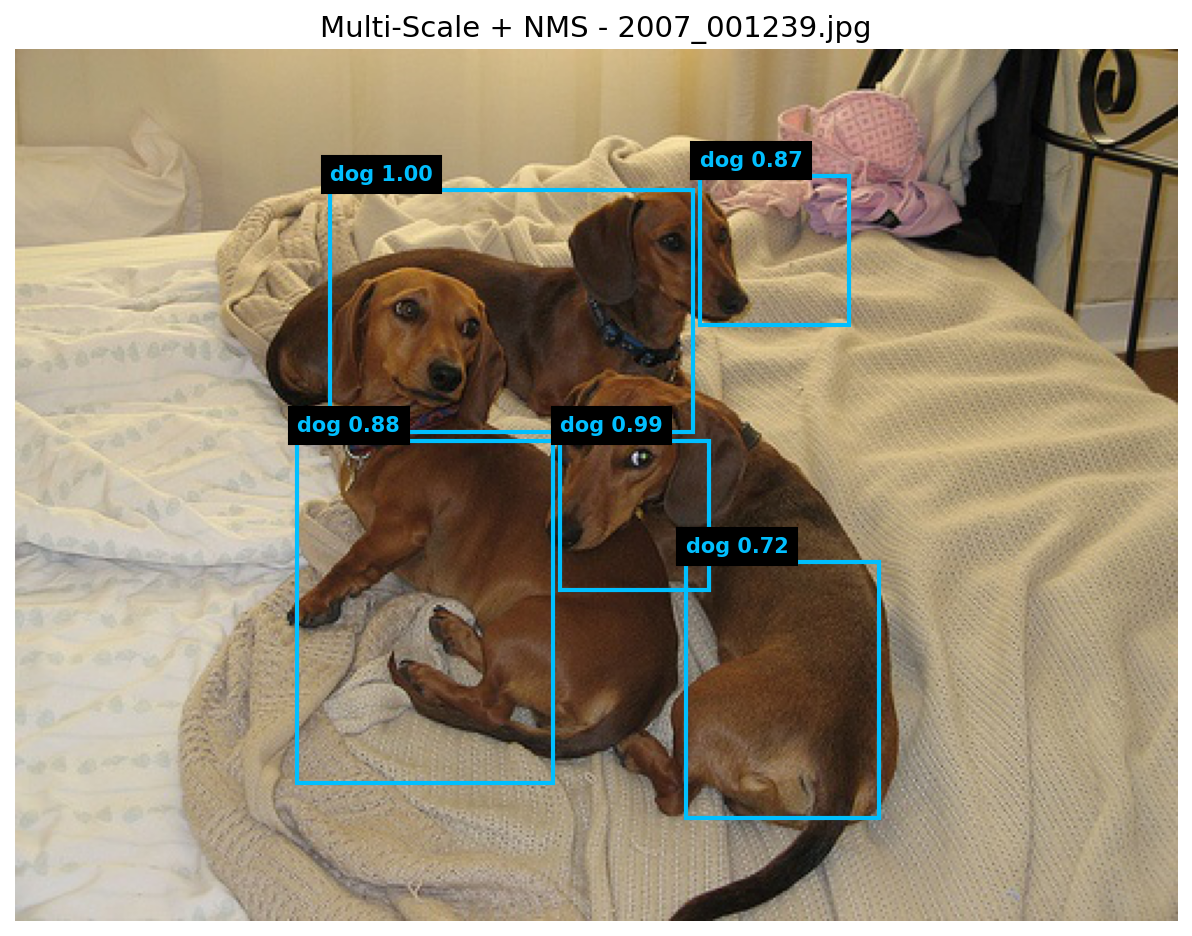
\includegraphics[width=\linewidth]{results/q3_improved_2007_001239.png}
        \caption{Proposed on Image 1}
    \end{minipage}\hfill
    \begin{minipage}{0.48\textwidth}
        \centering
        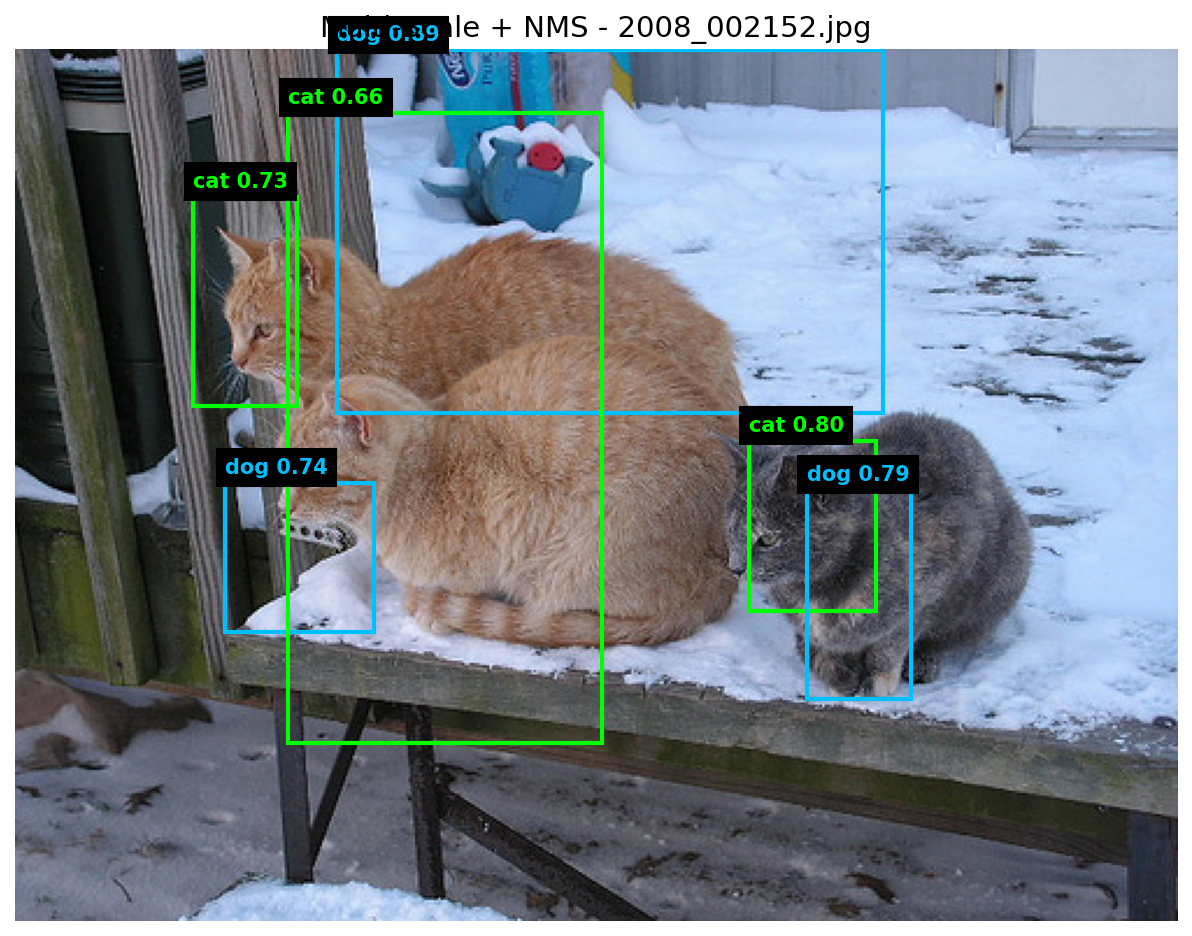
\includegraphics[width=\linewidth]{results/q3_improved_2008_002152.png}
        \caption{Proposed on Image 2}
    \end{minipage}
\end{figure}
As shown above, the proposed method easily outperformed the baseline method, with more accurate prediction regions and detection rate of cats.
\section{Deliverable 4: Performance Profiling}

The performance benchmarking profiling Faster-RCNN and YOLOv8n was calculated locally on COCO 2017 Val. 

\begin{figure}[H]
    \centering
    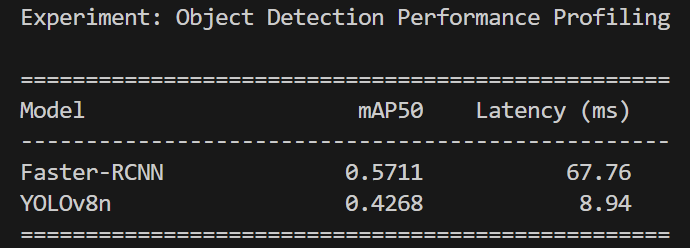
\includegraphics[width=0.8\linewidth]{results/q4.png}
    \caption{Performance Benchmarking Profiling on Faster-RCNN and YOLOv8n}
\end{figure}

Faster-RCNN, despite having significantly lower inference speeds due to region generation, outperforms YOLOv8n in accuracy thresholds strongly by around +14\% on the mAP50 metric. YOLO trades accuracy for extremely lower latency for real-time inference. 

\section{Modern Open Vocabulary Object Detection}

\subsection*{(a) YOLOv8s-world}
\begin{itemize}
    \item \textbf{mAP50 Validation:} Using \texttt{yolov8s-world.pt}, prompted solely with the exact MS COCO class names, we obtained the mAP50 of \textbf{0.4455} on the COCO 2017 validation splits.

    \item \textbf{Sample Testing:} As shown in Fig.\ref{fig:17}, the model performed relatively accurate predictions on the given samples. 
\end{itemize}

\begin{figure}[H]
    \centering
    \begin{minipage}{0.48\textwidth}
        \centering
        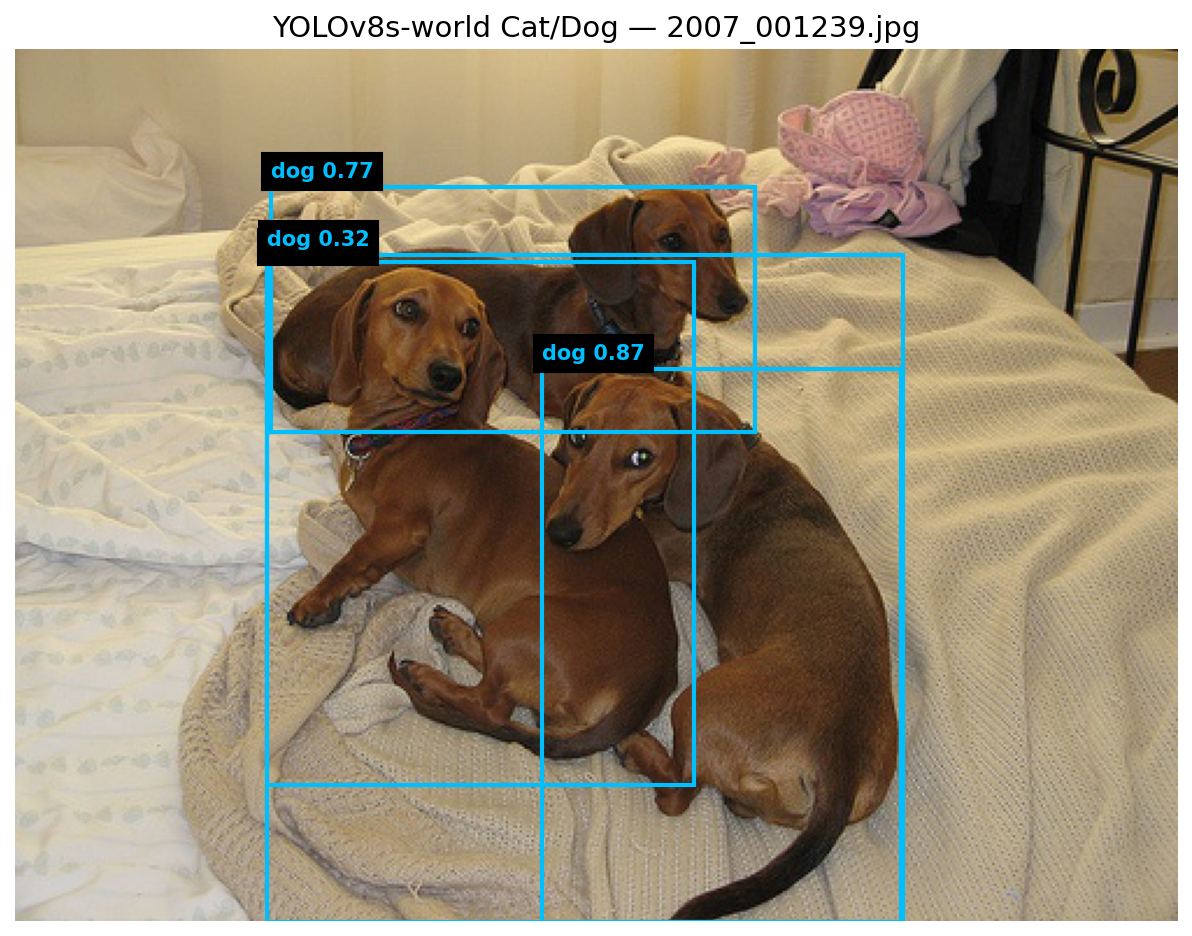
\includegraphics[width=\linewidth]{results/q5_catdog_2007_001239.png}
    \end{minipage}\hfill
    \begin{minipage}{0.48\textwidth}
        \centering
        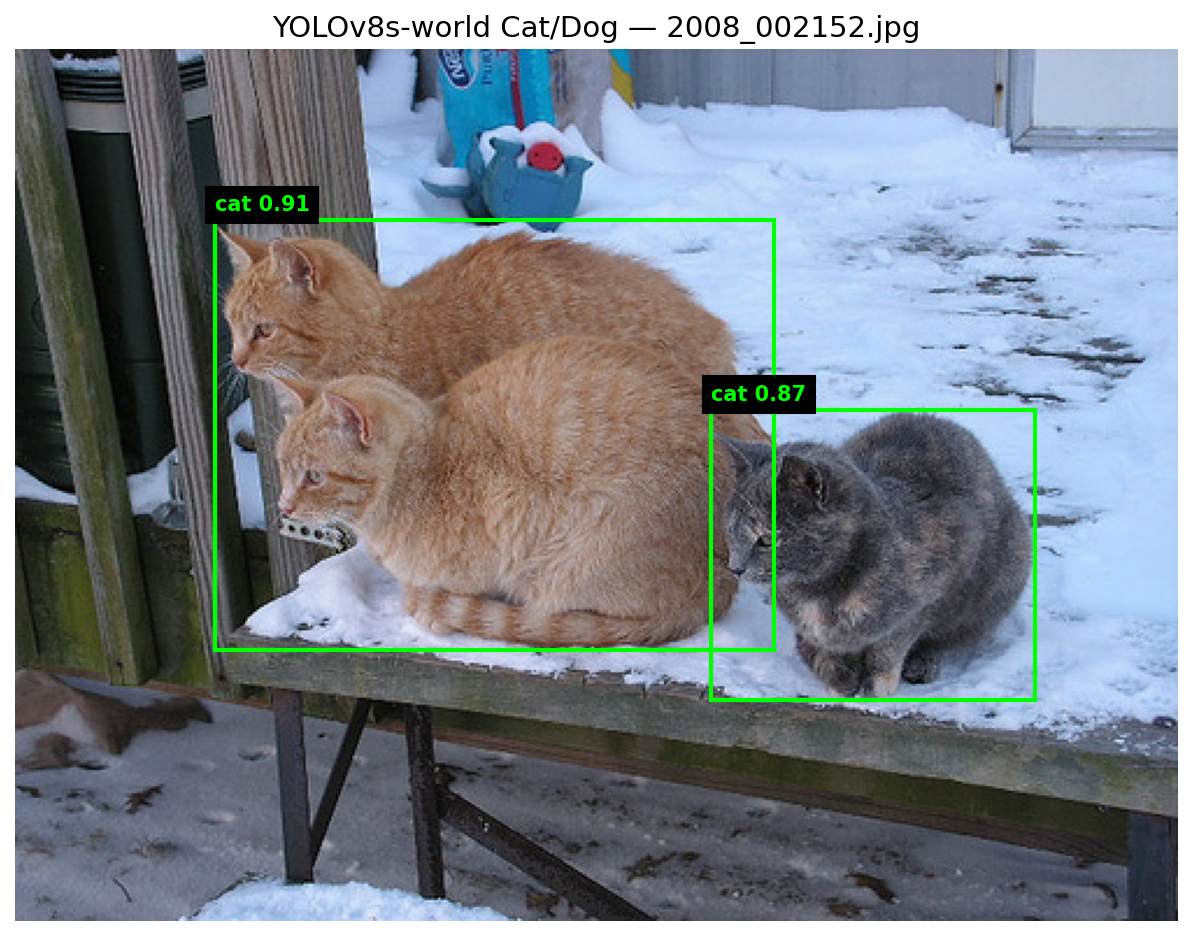
\includegraphics[width=\linewidth]{results/q5_catdog_2008_002152.png}
    \end{minipage}
    \caption{YOLOv8s-world Predictions on Cats and Dogs}
    \label{fig:17}
\end{figure}

\begin{figure}[H]
    \centering
    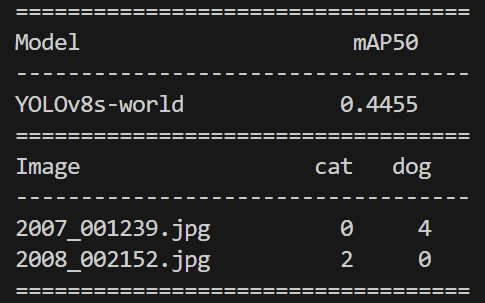
\includegraphics[width=0.5\linewidth]{results/q5_log.png}
    \caption{YOLOv8s-world Inference Summary}
\end{figure}

\subsection*{(b) Large Vision Language Models}
I utilize Gemini 3.1 Pro to perform the detection task.

\subsubsection*{Prompt}
\begin{lstlisting}
Detect cats and dogs in the provided images. Please directly draw the bounding boxes and corresponding labels on the corresponding graph. Do not give me the bboxes in json.
\end{lstlisting}

\subsubsection*{Full Response}
Gemini automatically invoked the Create Image feature and responded directly with the required image, without text response:
\begin{figure}[H]
    \centering
    \includegraphics[width=0.8\linewidth]{results/q5_Gemini_Generated_Image_gzkeuygzkeuygzke.png}
    \caption{Visual Bounding Boxes Output generated by Gemini Vision Language Model}
\end{figure}

\end{document}